\documentclass[11pt]{article}
\usepackage[margin=1in]{geometry}
\usepackage[T1]{fontenc}
\usepackage{lmodern}
\usepackage{microtype}
\usepackage{amsmath,amssymb}
\usepackage{booktabs}
\usepackage{graphicx}
\usepackage[font=small,labelfont=bf]{caption}
\usepackage[numbers,sort&compress]{natbib}
\usepackage{xcolor}
\usepackage{tikz}
\usetikzlibrary{positioning,arrows.meta,calc}
\usepackage[colorlinks=true,linkcolor=teal!70!black,citecolor=teal!70!black,urlcolor=teal!70!black]{hyperref}

% Author and code link
\newcommand{\AuthorName}{Mohammad Alnajdawi}
\newcommand{\AuthorAffil}{Independent Researcher}
\newcommand{\AuthorEmail}{najdawimohamed@gmail.com}
\newcommand{\CodeURL}{\url{https://github.com/Mohamednajdawi/one-neuron-edit}}


\newcommand{\R}{\mathbb{R}}
\setlength{\emergencystretch}{1.5em}
\newcommand{\vect}[1]{\boldsymbol{#1}}
\definecolor{cbase}{HTML}{8c96a3}
\definecolor{cone}{HTML}{1f7a8c}
\definecolor{ctwo}{HTML}{0b3c49}
\definecolor{cD}{HTML}{c0392b}

\title{\textbf{One Neuron, One Bias Vector, No Training:}\\[2pt]
\large A Frontier LLM Edits 0.0002\% of a Language Model's Weights\\ and Recovers Hidden Accuracy on Medical Exam Questions}
\author{\AuthorName\thanks{The diagnosis, the analysis code and both weight edits reported here were produced by Claude Opus 5.5 (Anthropic) working as an AI agent. The author set the task, the budget and the follow-up requests (Table~\ref{tab:roles}).}\\ \AuthorAffil\\ \texttt{\AuthorEmail}}
\date{}

\begin{document}
\maketitle

\begin{abstract}
Can a frontier language model improve another model on a real benchmark by reading and rewriting its weights, with no training? We gave Claude Opus 5.5, working as a coding agent at maximum reasoning effort, the task of improving Qwen2.5-0.5B-Instruct on MedMCQA, a benchmark of medical entrance-exam questions, by editing at most 4\% of its weights. Zero-shot, Qwen answers ``D'' 75\% of the time although ``D'' is correct only 20\% of the time, and scores 28.9\%, below always answering ``A'' (30.9\%). Within 30 minutes, the agent used a logit lens and direct logit attribution to trace this habit to the last three blocks and to a single MLP neuron (block~21, neuron~2921) that adds $+2.04$ logits to ``D'', 2.8 times more than any other of the model's 116{,}736 MLP neurons. It then wrote a two-part edit: an orthogonal projection that removes the neuron's letter-voting component, and a closed-form counterweight in block~23's value bias, fitted on unlabeled questions. The edit changes 1{,}015 of 494 million weights (0.0002\%) and uses no gradients and no labels. On 9{,}183 held-out questions, accuracy rises from 28.9\% to 35.5\% (McNemar $p=1.1\times10^{-36}$), answer consistency under option reordering doubles, and the loss on medical prose changes by only 0.16\%. The edit adds no medical knowledge: accuracy averaged over option orders stays at 36.5\%. Asked to improve further, the agent selected a second edit using labels; it gained 1.6 points on its selection set but only 0.16 points on held-out data ($p=0.45$), a winner's curse. In this case study, LLM-driven weight editing removed an obstacle that hid an ability but did not add one, and only untouched data told the two apart.
\end{abstract}

% =====================================================================
\section{Introduction}

Recent work argues that frontier large language models (LLMs) can read and write neural-network weights directly, a capability its authors call \emph{weight-space programming} \citep{takehi2026weightspace}. In their most striking experiment, a frontier model edited 0.016\% of the weights of Qwen3.5-0.8B without any training, removing a direction that caused reasoning loops and raising MATH-500 accuracy from 7.9\% to 48.1\%. The same study reports the opposite case: for a model whose errors had no single cause, the edits did not help. The authors conclude: ``Editing weights could remove an obstacle that hid an ability, but it could not add an ability the model lacked.''

We test this with a publicly available frontier model on a standard benchmark, and ask whether the gains survive held-out evaluation. We gave Claude Opus 5.5, running as a coding agent, a small instruction-tuned model, Qwen2.5-0.5B-Instruct \citep{qwen2024qwen25}, and a medical multiple-choice benchmark, MedMCQA \citep{pal2022medmcqa}, with one instruction: edit the weights to improve the results. The author suggested no method, component or weight (Table~\ref{tab:roles}).

The model turned out to have an extreme case of a known failure, \emph{selection bias}: a preference for particular option letters regardless of content \citep{zheng2024selectors,pezeshkpour2024order}. Standard remedies act from the outside, recalibrating output probabilities \citep{zhao2021calibrate} or permuting the options and averaging \citep{zheng2024selectors}, at every inference call. The agent instead located the bias inside the network and removed it there, permanently, with an edit small enough to print in full (Figure~\ref{fig:teaser}).

\begin{figure}[t]
\centering
\resizebox{\textwidth}{!}{%
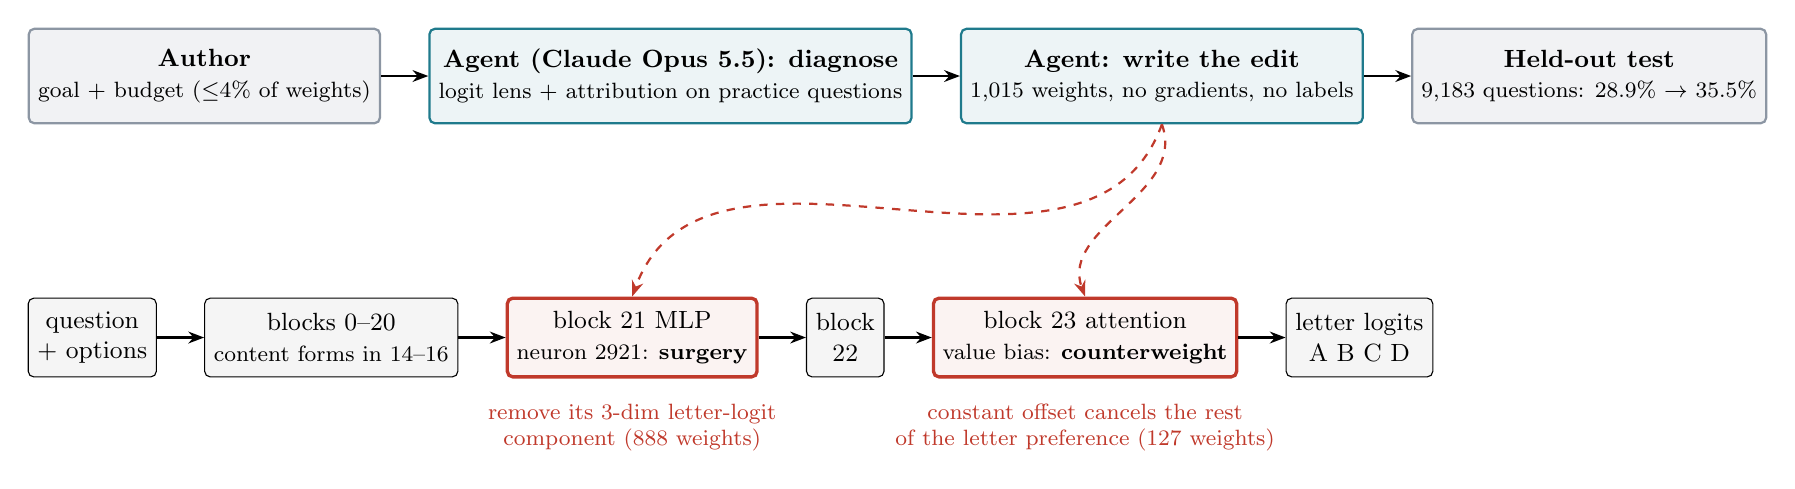
\begin{tikzpicture}[
  node distance=6mm, font=\small,
  blk/.style={draw, rounded corners=2pt, minimum height=10mm, align=center, fill=gray!8},
  edit/.style={draw=cD, very thick, rounded corners=2pt, minimum height=10mm, align=center, fill=cD!6},
  agentbox/.style={draw=cone, thick, rounded corners=2pt, minimum height=12mm, align=center, fill=cone!8},
  person/.style={draw=cbase, thick, rounded corners=2pt, minimum height=12mm, align=center, fill=cbase!12},
  note/.style={align=center, font=\footnotesize, text=cD},
  arr/.style={-{Stealth[length=2mm]}, thick}]
\node[person] (task) {\textbf{Author}\\ \footnotesize goal + budget ($\le$4\% of weights)};
\node[agentbox, right=of task] (diag) {\textbf{Agent (Claude Opus 5.5): diagnose}\\ \footnotesize logit lens + attribution on practice questions};
\node[agentbox, right=of diag] (write) {\textbf{Agent: write the edit}\\ \footnotesize 1{,}015 weights, no gradients, no labels};
\node[person, right=of write] (test) {\textbf{Held-out test}\\ \footnotesize 9{,}183 questions: 28.9\% $\to$ 35.5\%};
\draw[arr] (task) -- (diag); \draw[arr] (diag) -- (write); \draw[arr] (write) -- (test);
\node[blk, below=22mm of task.south west, anchor=north west] (in) {question\\ + options};
\node[blk, right=of in] (mid) {blocks 0--20\\ \footnotesize content forms in 14--16};
\node[edit, right=of mid] (b21) {block 21 MLP\\ \footnotesize neuron 2921: \textbf{surgery}};
\node[blk, right=of b21] (b22) {block\\ 22};
\node[edit, right=of b22] (b23) {block 23 attention\\ \footnotesize value bias: \textbf{counterweight}};
\node[blk, right=of b23] (out) {letter logits\\ A B C D};
\draw[arr] (in) -- (mid); \draw[arr] (mid) -- (b21); \draw[arr] (b21) -- (b22); \draw[arr] (b22) -- (b23); \draw[arr] (b23) -- (out);
\node[note, below=2mm of b21] {remove its 3-dim letter-logit\\ component (888 weights)};
\node[note, below=2mm of b23] {constant offset cancels the rest\\ of the letter preference (127 weights)};
\draw[-{Stealth[length=2mm]}, dashed, cD, thick] (write.south) to[out=-110, in=70] (b21.north);
\draw[-{Stealth[length=2mm]}, dashed, cD, thick] (write.south) to[out=-70, in=110] (b23.north);
\end{tikzpicture}}
\caption{\textbf{What happened, and what changed.} \emph{Top:} the author set a goal and a budget; Claude Opus 5.5, working as a coding agent, diagnosed the model and wrote the edit using practice questions only; the edit was then scored on held-out questions. \emph{Bottom:} the two tensors the agent changed: one column of block 21's MLP down-projection (888 weights) and block 23's value bias (127 weights).}
\label{fig:teaser}
\end{figure}

\paragraph{Contributions.}
\begin{enumerate}
\item \textbf{A documented case of LLM-driven weight editing on a real benchmark.} We report what the agent was told, what it did, and when (Table~\ref{tab:roles}, Appendix~\ref{app:prompts}). About 70 minutes after receiving the task, it had saved an edit of 1{,}015 weights and scored it on held-out questions.
\item \textbf{The mechanism it found and the edit it wrote} (\S\ref{sec:diagnosis} and \S\ref{sec:method}). Answer content forms in blocks 14--16; a ``D'' preference is added in blocks 21--23, much of it by one neuron. The edit combines an orthogonal projection of that neuron's output vector with a closed-form value-bias counterweight.
\item \textbf{Held-out evaluation} on 9{,}183 questions never used for design: +6.6 accuracy points, doubled consistency under option reordering, and a negligible change on medical prose (\S\ref{sec:results}).
\item \textbf{Two negative results that bound the claim.} The edit recovers accuracy the model already had but adds none (\S\ref{sec:ceiling}), and the agent's second, label-selected edit looked significant on its selection set but vanished on held-out data (\S\ref{sec:round2}). For an agent that edits weights, the evaluation protocol matters as much as the edit.
\end{enumerate}

% =====================================================================
\section{Related work}

\paragraph{Weight-space programming.} \citet{takehi2026weightspace} show frontier LLMs reading weights (e.g., telling which game a policy network was trained on) and writing them (fixing a failing controller, writing game-playing networks from scratch, and removing a looping direction from Qwen3.5-0.8B). We study one such edit end to end, with a publicly available model, a standard benchmark, held-out test sets and paired statistical tests.

\paragraph{Selection bias in MCQ answering.} LLMs prefer specific option IDs \citep{zheng2024selectors} and are sensitive to option order \citep{pezeshkpour2024order}. \citet{robinson2023leveraging} show that the ability to bind answers to symbols (``multiple-choice symbol binding'') varies widely across models. Calibration with content-free inputs \citep{zhao2021calibrate} and accounting for surface-form competition \citep{holtzman2021surface} correct output distributions at inference time. The agent's counterweight is the weight-space analogue of content-free calibration, but it is estimated from real questions in all four orders rather than from a null prompt, and it is written once into the weights.

\paragraph{Mechanisms of MCQ answering.} \citet{lieberum2023circuit} identify ``correct-letter'' attention heads in Chinchilla 70B. \citet{wiegreffe2025answer} find that answer-symbol prediction is causally attributable to a few middle layers and that later layers amplify the chosen symbol through a sparse set of heads. Our lens results agree with this picture (content in middle layers, amplification later) and add that, in a small model, the late layers also inject a large content-independent bias.

\paragraph{Reading and editing components.} The agent used the logit lens \citep{nostalgebraist2020logitlens,belrose2023tuned} and direct logit attribution in the residual-stream view of transformers \citep{elhage2021framework}. Treating MLP neurons as key-value memories whose output vectors promote vocabulary items \citep{geva2021keyvalue,geva2022promoting} makes a single neuron's ``vote'' on the letters directly computable. \citet{stolfo2024confidence} describe neurons that shift outputs toward token-frequency priors, a phenomenon related to the habit neuron we find. Weight editing has been used to change facts \citep{meng2022rome,meng2023memit}; directional ablation removes behaviors mediated by a single direction \citep{arditi2024refusal}. The agent's surgery is a directional ablation restricted to one neuron and to the letter subspace only.

% =====================================================================
\section{Setup}
\label{sec:setup}

\paragraph{The agent.} Claude Opus 5.5 (Anthropic), at maximum reasoning effort, used through the agent mode of GitHub Copilot in Visual Studio Code on an Apple-silicon laptop with 64\,GB of memory. The agent could read and write files, run shell commands and Python (PyTorch, Hugging Face Transformers), and run the model forward on any question. There was no limit on forward passes and, as in the weight-space programming setting, no gradient-based training. All work took place in one conversation with the author (November 4--6, 2026).

\paragraph{The task.} The author's instructions are reproduced in Appendix~\ref{app:prompts}. In short: measure the baseline of Qwen2.5-0.5B-Instruct on MedMCQA, then edit its weights to improve the results, changing at most 4\% of them (a budget set earlier in the conversation). After Edit 1 was saved, the author asked for a before-and-after test on 5{,}000 more questions, for an answer-consistency analysis, and for a second round of edits, tested on 1{,}000 questions first and then on the rest.

\paragraph{Rules the agent adopted.} Beyond the budget, the agent imposed on itself: no changes to the embeddings, the output head or the final normalization; no rescaling of whole tensors; all analysis and selection on practice questions; and each test set scored once per edit.

\begin{table}[t]
\centering\small
\caption{\textbf{Who did what.} The author never suggested a method, a component or a weight.}
\label{tab:roles}
\begin{tabular}{p{0.44\textwidth}p{0.48\textwidth}}
\toprule
Author (human) & Agent (Claude Opus 5.5) \\
\midrule
Chose the model and the benchmark; pointed the agent to the weight-space programming post. & Wrote all code: data loading, splits, scoring, analysis, edits, statistics and figures. \\
Set the goal (improve accuracy by editing the weights) and the budget (at most 4\% of the weights). & Designed the evaluation: practice questions for all analysis and selection, separate test sets, rotation-balanced scoring. \\
Asked for a test on 5{,}000 more questions and for an answer-consistency analysis. & Diagnosed the failure (logit lens, attribution) and found neuron 2921. \\
Asked for a second round of edits, tested on 1{,}000 questions first, then on the rest. & Designed and applied both edits, selected Edit 2, and ran all evaluations. \\
Reviewed the results and this manuscript. & Ran the later checks (order-averaged lens, probes, ablation) and drafted this manuscript. \\
\bottomrule
\end{tabular}
\end{table}

\paragraph{Model.} Qwen2.5-0.5B-Instruct: 494{,}032{,}768 parameters, 24 blocks, residual width $d=896$, 14 query heads of size 64 sharing 2 key-value groups, MLP width 4{,}864, tied input/output embeddings, final RMSNorm. Weights are used in bfloat16.

\paragraph{Protocol.} The agent presented each question zero-shot through the model's chat template (with its default system prompt) as: \emph{``Answer the following multiple choice question. Reply with only the letter (A, B, C, or D) of the correct option.''} followed by the question and four lettered options. The prediction is the argmax of the next-token logits restricted to the tokens ``A''--``D''. On average these four tokens carry 81\% of the next-token probability mass, so the restriction rarely changes the choice. All scoring uses batch size 1 and is deterministic. MedMCQA questions are of two kinds, single-concept and combination (``multi'') questions; both are included.

\paragraph{Data splits (Table~\ref{tab:splits}).} MedMCQA's validation split consists of NEET PG exam questions, and its training split of mock and online test series \citep{pal2022medmcqa}; the official test labels are not public. The agent therefore used the full validation split as a \emph{real-exam test} and 5{,}000 further training questions as a \emph{mock-exam test}. The agent did all analysis, design and selection on a separate \emph{practice} set of 4{,}000 training questions, de-duplicated against both test sets by question text, and scored the test sets only after an edit was fixed.

\begin{table}[t]
\centering\small
\caption{\textbf{Data splits.} All edit design used practice questions only; the calibration subset is used without labels.}
\label{tab:splits}
\begin{tabular}{llrl}
\toprule
Name & Source (MedMCQA split) & $n$ & Use \\
\midrule
Analysis & train (practice 0--1{,}499) & 1{,}500 & lens, attribution, neuron selection \\
Calibration & train (practice 0--499) & 500 & counterweight fit (labels unused) \\
Tryout & train (practice 3{,}000--3{,}999) & 1{,}000 & comparing candidate edits \\
\midrule
Real-exam test & validation (NEET PG) & 4{,}183 & held out \\
Mock-exam test & train (disjoint from practice) & 5{,}000 & held out; also scored in 4 orders \\
\bottomrule
\end{tabular}
\end{table}

\paragraph{Metrics and statistics.} We report accuracy with Wilson 95\% intervals \citep{wilson1927}. Paired comparisons between models on the same questions use the exact two-sided McNemar test \citep{mcnemar1947} on the counts of questions \emph{fixed} (wrong$\to$right) and \emph{broken} (right$\to$wrong); paired intervals for an accuracy difference use $\Delta=(f-b)/n$ with standard error $\sqrt{f+b-(f-b)^2/n}\,/\,n$. On the mock-exam test we also present each question in all four cyclic option orders ($\pi_k$: ABCD, BCDA, CDAB, DABC) and report: \emph{rotation-balanced accuracy} (mean over orders), \emph{consistency} (how many of the four orders select the same underlying option), and the \emph{four-order ensemble} (argmax of the per-option log-probabilities averaged over orders). Because each option appears under each letter exactly once, these quantities are insensitive to letter preferences.

\paragraph{Notation.} Let $\vect{x}\in\R^d$ be the final residual stream at the answer position, $\vect{g}$ the final RMSNorm gain, $r=\mathrm{rms}(\vect{x})$, and $U\in\R^{4\times d}$ the matrix whose rows are $(\vect{u}_c\odot\vect{g})^\top$ for the unembedding vectors $\vect{u}_c$ of letters $c\in\{A,B,C,D\}$. The letter logits are $\vect{\ell}=U\vect{x}/r$. Only differences between letter logits matter, so we work with $C\vect{\ell}$, where $C=I-\tfrac14\mathbf{1}\mathbf{1}^\top$. Empirically $r=1.54\pm0.04$ across questions, so $r$ is well approximated by a constant $\bar r$.

% =====================================================================
\section{Diagnosis: what the agent found}
\label{sec:diagnosis}

\begin{figure}[t]
\centering
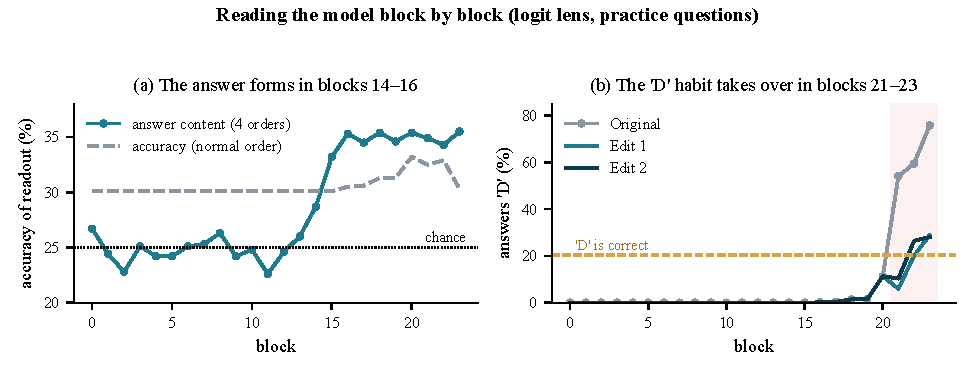
\includegraphics[width=\textwidth]{figures/fig_lens.pdf}
\caption{\textbf{Reading the model block by block.} Logit lens on 1{,}000--1{,}500 practice questions. (a) Answer content per block, measured by reading the letter logits from the residual stream after each block and averaging per-option log-probabilities over the four cyclic option orders (solid), versus plain accuracy in the normal order (dashed). Content appears in blocks 14--16 and is preserved to the output. (b) Share of questions answered ``D'' when read after each block. In the original model the ``D'' share jumps in blocks 21--23 (shaded); both edits remove most of this jump.}
\label{fig:lens}
\end{figure}

\paragraph{What the agent measured before editing.} Before changing any weight, the agent scored the baseline, scored 1{,}000 practice questions in all four option orders, read the letter logits after every block (a logit lens, in the normal option order), and computed the direct logit attribution of every attention head and MLP neuron on 1{,}500 practice questions. It named neuron 2921 thirty minutes after receiving the task. The order-averaged lens (Figure~\ref{fig:lens}a), the linear probes and the per-neuron statistics reported below were computed after both edits, as checks on this diagnosis.

\paragraph{The model knows more than it says.} On the 9{,}183 test questions, the original model predicts (A, B, C, D) in $(13.2, 4.2, 7.2, 75.4)\%$ of cases, while the correct letters occur in $(30.9, 26.2, 22.4, 20.4)\%$. Its accuracy is 86.2\% when the answer is ``D'' and 7.8\% when it is ``B''. Yet the four-order ensemble, which cancels letter preferences, reaches 36.5\% on the mock-exam test (measured after the edits), 7 points above the model's normal-order accuracy. Answering ``D'' is a habit layered on top of a better underlying answer.

\paragraph{Answer content forms in the middle; the habit is added at the end.} Reading the letter logits after every block (Figure~\ref{fig:lens}a), order-averaged content stays at chance (22.6--26.7\%) through block 13, rises to 33.2\% at block 15 and 35.3\% at block 16, and stays between 34.3\% and 35.5\% until the output. In the normal order, the ``D'' share is at most 1.4\% through block 19 and 11.3\% at block 20, then jumps to 54.1\%, 59.5\% and 75.8\% after blocks 21, 22 and 23 (Figure~\ref{fig:lens}b). The answer is decided long before the habit takes over.

\paragraph{Later checks agree.} Linear probes (run after the edits), fit on 800 practice questions and tested on 400 others (all in four orders), decode the displayed correct letter from the residual stream with at most 34.9\% accuracy (block 23), against 30.6\% for a control probe that sees only option lengths. The information the probes find does not exceed what the order-averaged readout already exposes, so we treat $\approx$35--36\% as the model's own ceiling under this protocol.

\paragraph{The habit is a constant offset.} At the output, the letter logits contain a mean centered offset of $(-0.22,-1.06,-0.17,+1.45)$ for (A, B, C, D) on top of a content signal that raises the correct letter by $+0.32$ logits on average. Subtracting the constant offset alone (an oracle that uses the analysis set's mean) raises analysis-set accuracy to 34.3\%.

\begin{figure}[t]
\centering
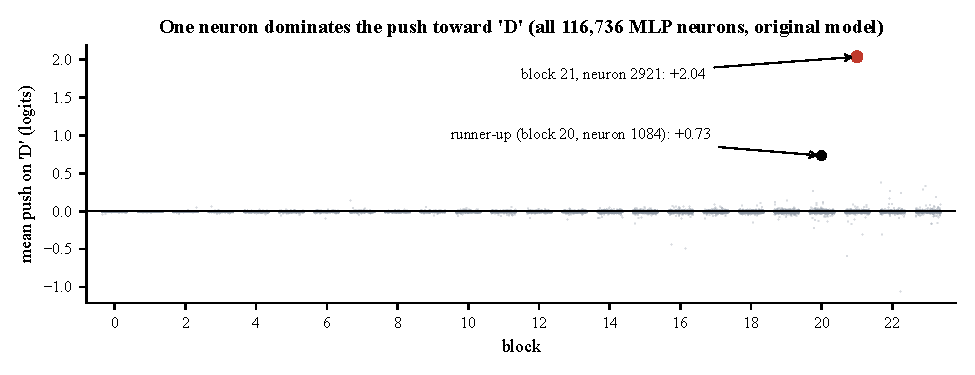
\includegraphics[width=\textwidth]{figures/fig_neurons.pdf}
\caption{\textbf{One neuron dominates the push toward ``D''.} Mean centered push on the ``D'' logit for every one of the 116{,}736 MLP neurons (direct logit attribution, analysis set), by block. One neuron stands out: block 21, neuron 2921 (+2.04 logits). The runner-up anywhere in the network is 2.8 times smaller.}
\label{fig:neurons}
\end{figure}

\paragraph{One neuron carries most of it.} The agent's direct logit attribution decomposes $C\vect{\ell}$ into contributions of every attention head and MLP neuron, holding $r$ at its observed value. The neuron $j$ of block $l$ contributes $a_{l,j}\,CU\vect{w}_{l,j}/r$, where $a_{l,j}$ is its activation and $\vect{w}_{l,j}$ its output vector (a column of the down-projection). Over the analysis set, neuron 2921 of block 21 contributes a mean centered vote of $(-0.59,-0.80,-0.65,+2.04)$ (Figure~\ref{fig:neurons}), and the agent chose it as the target of its edit. Statistics computed later confirm the picture: it is active on 99.7\% of questions (mean activation $4.77\pm1.57$); its ``D'' vote is $2.04\pm0.67$ logits. That vote is mildly larger when ``D'' is in fact correct (correlation 0.21), so the neuron is mostly habit with a small amount of signal. The next-largest ``D''-pushing neuron in the whole network (block 20, neuron 1084) contributes $+0.73$; within block 21 the runner-up contributes $+0.09$. Among attention heads, the largest ``D'' pushes come from heads 16.11 ($+0.83$), 16.7 ($+0.57$) and 21.9 ($+0.49$), but these are spread over several heads and blocks, and block 16's attention push is partly cancelled by its own MLP ($-0.84$). Summed over all components, the attributed ``D'' push is $+1.48$, matching the observed offset of $+1.45$.

% =====================================================================
\section{Method: the agent's edit}
\label{sec:method}

The agent's edit has two parts (Figure~\ref{fig:teaser}, bottom).

\paragraph{Neuron surgery.} The letter-logit differences depend on $\vect{x}$ only through $CU\vect{x}$, a rank-3 map. Let $Q\in\R^{d\times3}$ be an orthonormal basis of the row space of $CU$ (from its singular value decomposition). The agent replaced the neuron's output vector by
\begin{equation}
\vect{w}_{21,2921}\;\leftarrow\;(I-QQ^\top)\,\vect{w}_{21,2921}.
\end{equation}
Since $CU(I-QQ^\top)=0$, the neuron's direct vote on letter differences becomes exactly zero, while its remaining 893-dimensional component, which may serve other purposes, is untouched. The projection removes 35\% of the vector's squared norm and changes 888 of its 896 entries at bfloat16 precision. Surgery alone moves the content-free letter preference on calibration questions from $(16.2, 8.2, 15.9, 59.7)\%$ to $(23.2, 12.3, 24.8, 39.8)\%$: it removes about half of the excess ``D'' preference, but not all of it, because the habit has other, smaller sources.

\paragraph{Counterweight.} To cancel the remaining preference without touching any other neuron, the agent used the value bias of block 23's attention. Let $\mathcal G_k$ be the 7 query heads that share key-value group $k\in\{1,2\}$, $O_h\in\R^{d\times64}$ the slice of the output projection for head $h$, and $\vect b_k\in\R^{64}$ the value bias of group $k$. Because each head's attention weights sum to one, a change $\Delta\vect b$ of the value bias reaches the residual stream unchanged at \emph{every} position:
\begin{equation}
\Delta\vect o_t=\sum_h O_h\sum_s \alpha^h_{ts}\,\Delta\vect b_{k(h)}=M\,\Delta\vect b,\qquad M=\Big[\textstyle\sum_{h\in\mathcal G_1}O_h,\;\sum_{h\in\mathcal G_2}O_h\Big]\in\R^{d\times128}.
\end{equation}
Block 23 is the last block, so to first order the letter logits move by $C\Delta\vect\ell\approx CUM\Delta\vect b/\bar r$. It measured the \emph{content-free letter preference} $\bar{\vect p}$, the letter distribution averaged over the 500 calibration questions and their four cyclic orders,
\begin{equation}
\bar p_c=\frac{1}{4N}\sum_{i=1}^{N}\sum_{k=1}^{4}\mathrm{softmax}\big(\vect\ell(x_i^{\pi_k})\big)_c,
\end{equation}
which would be uniform for a model without letter preferences, and solved for the minimum-norm bias change that cancels it:
\begin{equation}
\Delta\vect b=\Big(\frac{CUM}{\bar r}\Big)^{+}C\,(-\log\bar{\vect p}).
\end{equation}
Because the linearization is approximate, it repeated measurement and solution three times. The preference before rounds 2 and 3 is $(25.1,18.1,26.2,30.6)\%$ and $(25.5,21.4,26.1,27.0)\%$, and close to uniform after. No labels are used. The final change has norm 2.36 (the original bias has norm 16.7), changes 127 of the 128 entries, and injects a constant centered offset of $(-0.05,+1.09,-0.19,-0.85)$ logits.

\paragraph{Timeline.} The agent wrote the code for both parts within three minutes of naming the neuron. Before saving the edit, it compared four variants (no edit, surgery only, counterweight only, both) on the tryout set, by accuracy only. It scored the final edit on the 4{,}183 real-exam questions and saved it 69 minutes after receiving the task (Appendix~\ref{app:prompts}). The 1{,}015 changed weights (0.0002\% of the model) are far within the 4\% budget.

% =====================================================================
\section{Results}
\label{sec:results}

\begin{table}[t]
\centering\small
\caption{\textbf{Held-out results.} Accuracy (\%) with the half-width of the 95\% interval. Edit 2 is described in \S\ref{sec:round2}. ``Always A'' scores 32.2 (real-exam), 29.9 (mock-exam) and 30.9 (both). Medical-text loss is the mean next-token loss on 200 MedMCQA expert explanations (ordinary prose, not MCQs).}
\label{tab:main}
\begin{tabular}{lccc}
\toprule
 & Original & Edit 1 & Edit 2 \\
\midrule
Weights changed & 0 & 1{,}015 & 1{,}905 \\
Real-exam test ($n$=4{,}183) & 28.1 {\scriptsize$\pm$1.4} & 34.4 {\scriptsize$\pm$1.4} & 34.7 {\scriptsize$\pm$1.4} \\
Mock-exam test ($n$=5{,}000) & 29.6 {\scriptsize$\pm$1.3} & 36.4 {\scriptsize$\pm$1.3} & 36.4 {\scriptsize$\pm$1.3} \\
\quad rotation-balanced & 31.8 {\scriptsize$\pm$0.7} & 34.8 {\scriptsize$\pm$0.9} & 34.8 {\scriptsize$\pm$0.9} \\
Both tests ($n$=9{,}183) & 28.9 {\scriptsize$\pm$0.9} & \textbf{35.5} {\scriptsize$\pm$1.0} & 35.6 {\scriptsize$\pm$1.0} \\
\midrule
Fixed / broken vs.\ Original & -- & 1{,}447 / 844 & 1{,}492 / 874 \\
McNemar $p$ vs.\ Original & -- & $1.1\times10^{-36}$ & $2.8\times10^{-37}$ \\
Fixed / broken vs.\ Edit 1 & -- & -- & 181 / 166 ($p$=0.45) \\
Medical-text loss (nats/token) & 3.045 & 3.050 & 3.058 \\
\bottomrule
\end{tabular}
\end{table}


\begin{figure}[t]
\centering
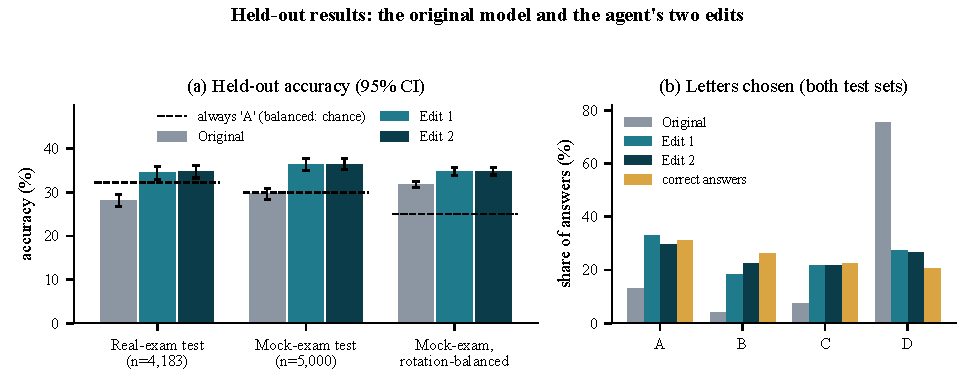
\includegraphics[width=\textwidth]{figures/fig_results.pdf}
\caption{\textbf{Held-out results.} (a) Held-out accuracy with 95\% intervals. Dashed lines: always answering ``A'' (chance, 25\%, for the rotation-balanced score). (b) Letters chosen on the 9{,}183 test questions, compared with the distribution of correct answers.}
\label{fig:results}
\end{figure}

\paragraph{Accuracy.} The agent scored Edit 1 on the real-exam test when it saved the edit; the mock-exam test and the consistency analysis were added later at the author's request, without changing the edit. Table~\ref{tab:main} and Figure~\ref{fig:results}a summarize the held-out results. Edit 1 raises accuracy from 28.1\% to 34.4\% on the real-exam test (641 fixed, 376 broken, $p=8.4\times10^{-17}$) and from 29.6\% to 36.4\% on the mock-exam test (806/468, $p=2.1\times10^{-21}$); over all 9{,}183 questions, from 28.9\% to 35.5\% ($p=1.1\times10^{-36}$). The original model is \emph{below} the always-``A'' baseline; the edited model is 4.5 points above it.

\paragraph{What is fixed and what is broken.} The edit breaks 844 answers, but 96.1\% of them have ``D'' as the correct answer: they were correct only because the model always says ``D''. Accuracy by correct letter changes from $(20.1,7.8,13.7,86.2)\%$ to $(41.7,26.7,30.4,42.8)\%$. The predicted letters move from $(13.2,4.2,7.2,75.4)\%$ to $(32.9,18.3,21.5,27.3)\%$ (Figure~\ref{fig:results}b), close to the true distribution.

\paragraph{The gain survives option reordering.} An edit that merely swapped one letter preference for another would show no gain on the rotation-balanced score. On the mock-exam test this score rises from 31.8\% to 34.8\% (paired difference $+3.0\pm0.6$ points, $z=9.4$). Per order, the original model ranges from 29.6\% to 35.1\% depending on where the correct answer lands; Edit 1 ranges from 33.3\% to 36.4\%.

\begin{figure}[t]
\centering
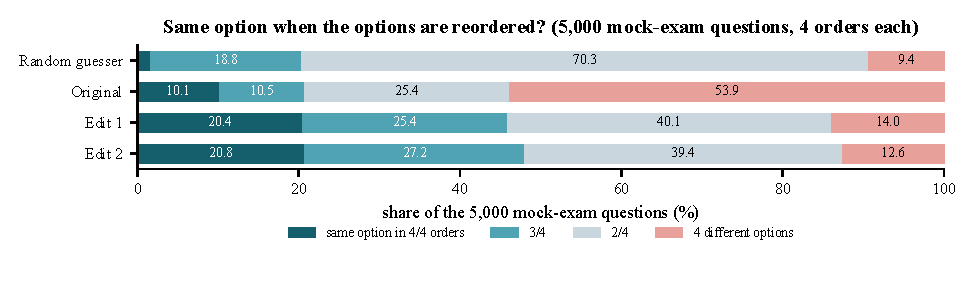
\includegraphics[width=\textwidth]{figures/fig_consistency.pdf}
\caption{\textbf{Consistency under option reordering} (mock-exam test): how many of the four cyclic option orders select the same underlying option. A uniform random guesser is shown for reference. The original model picks a different option in every order for 53.9\% of questions, far more often than a random guesser (9.4\%), because it follows the letter, not the option.}
\label{fig:consistency}
\end{figure}

\paragraph{Consistency.} The original model selects the same option in all four orders for only 10.1\% of questions and a different option in every order for 53.9\% (Figure~\ref{fig:consistency}), the signature of a model that tracks the letter rather than the content. After Edit 1, these become 20.4\% and 14.0\%. The share of questions answered correctly in all four orders rises from 6.4\% to 10.9\%.

\paragraph{Side effects.} The loss on 200 medical explanations changes from 3.0454 to 3.0503 nats per token (+0.16\%), and the probability mass on the four letter tokens from 0.81 to 0.78. The counterweight adds a constant offset to the letter logits at every position; we have not evaluated the edited model on other tasks in which ``A''--``D'' are frequent next tokens, and we note this as a limitation (\S\ref{sec:limitations}).

\paragraph{Ablation: what each part does.} While designing Edit 1, the agent compared surgery alone, the counterweight alone, and both on the tryout set; for this paper it re-ran the comparison with all metrics (Table~\ref{tab:ablation}). Surgery alone recovers about 40\% of the gain (2.1 of 5.2 points). The counterweight alone reaches the same accuracy as the full edit, as expected, since a constant offset can cancel any constant preference. However, it needs a bias change 1.7 times larger, injects a letter offset 1.8 times larger, and costs almost four times as much on medical prose (+0.61\% vs.\ +0.16\%). The surgery's value is therefore not accuracy but \emph{economy}: removing the main source makes the correction smaller and more local.

\begin{table}[t]
\centering\small
\caption{\textbf{What each part of Edit 1 does.} Ablation on the tryout set (1{,}000 practice questions, four orders each), run by the agent for this paper. ``Prior D'' is the content-free probability of ``D''; $\|\Delta\vect b\|$ is the norm of the value-bias change; ``Offset'' is the norm of the constant centered letter-logit offset it injects; ``Loss'' is the change in medical-text loss.}
\label{tab:ablation}
\begin{tabular}{lcccccccc}
\toprule
Variant & Acc. & Balanced & Same 4/4 & Diff.\ 4/4 & Prior D & $\|\Delta\vect b\|$ & Offset & Loss \\
\midrule
Original & 29.0 & 31.2 & 8.9 & 54.2 & 59.3 & 0 & 0 & -- \\
Surgery only & 31.1 & 33.4 & 15.0 & 26.4 & 39.5 & 0 & 0 & +0.01\% \\
Counterweight only & 34.2 & 34.5 & 20.1 & 17.7 & 27.6 & 4.09 & 2.56 & +0.61\% \\
Both (Edit 1) & 34.2 & 34.2 & 19.4 & 16.5 & 25.4 & 2.36 & 1.40 & +0.16\% \\
\bottomrule
\end{tabular}
\end{table}


% =====================================================================
\section{The ceiling: recovered, not created}
\label{sec:ceiling}

If the edit added medical knowledge, accuracy averaged over option orders, which is blind to letter preferences, would rise. It does not. The four-order ensemble scores 36.50\% for the original model, 36.52\% for Edit 1 and 36.46\% for Edit 2 on the mock-exam test. The paired rotation-balanced gain of +3.0 points comes from the original model's \emph{worst} orders (those that put the correct answer away from ``D''), not from new correct answers. The edit's single-pass accuracy (36.4\% in the normal order) approaches the four-order ensemble of the original model (36.5\%), at one quarter of the inference cost. This matches the lens (content $\approx$35.5\% at the output, Figure~\ref{fig:lens}a) and the probes (at most 34.9\%): the edit reveals accuracy that was present but hidden, and stops there. In the words of the hypothesis we set out to test \citep{takehi2026weightspace}, the edit removes an obstacle; it does not add an ability.

% =====================================================================
\section{The agent's second edit and the winner's curse}
\label{sec:round2}

\begin{figure}[t]
\centering
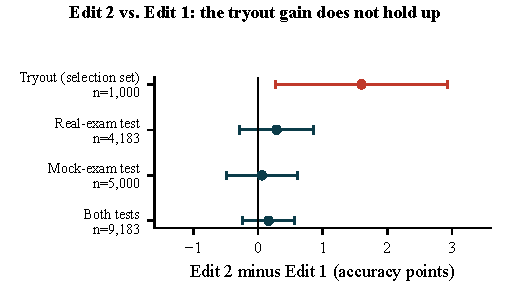
\includegraphics[width=0.55\textwidth]{figures/fig_round2.pdf}
\caption{\textbf{The winner's curse.} Edit 2 minus Edit 1 (accuracy points, paired 95\% intervals). The agent chose Edit 2 because it scored best on the tryout set (red). On held-out data the gain shrinks to near zero.}
\label{fig:round2}
\end{figure}

After Edit 1, the author asked whether editing about 1{,}000 more weights would improve the results, testing on 1{,}000 questions first. The agent looked for smaller, question-dependent letter votes that could also be removed profitably. Starting from Edit 1, for each of the 24{,}320 neurons in blocks 19--23 it computed, on the analysis set, the counterfactual letter logits if the neuron's \emph{question-to-question variation} in its letter vote were removed (its mean being re-absorbed by the counterweight),
\begin{equation}
\vect\ell'_i=\vect\ell_i-\big(\vect d_{ij}-\bar{\vect d}_j\big),\qquad
\mathrm{gain}_j=\frac1N\sum_i\Big[\log\mathrm{softmax}(\vect\ell'_i)_{y_i}-\log\mathrm{softmax}(\vect\ell_i)_{y_i}\Big],
\end{equation}
where $\vect d_{ij}$ is neuron $j$'s direct letter contribution on question $i$ and $y_i$ the correct letter. Unlike Edit 1, this criterion \emph{uses labels} and searches over tens of thousands of candidates. The agent applied the top three neurons (block 21, neurons 114, 407 and 717; estimated gains 0.044, 0.029 and 0.029 nats) and a ``re-calibrate only'' control for real (surgery, then a fresh 3-round counterweight) and compared them on the tryout set against Edit 1 (34.2\%): re-calibrate only 34.4\% (15 fixed/13 broken, $p=0.85$), neuron 407 34.6\%, neuron 717 34.7\%, and neuron 114 \textbf{35.8\%} (31/15, $p=0.026$). It adopted neuron 114 as Edit 2 (1{,}905 changed weights in total) and scored it once on the 1{,}000-question real-exam subset: +1.0 point over Edit 1 (23 fixed, 13 broken, $p=0.13$). At the author's request, it then scored Edit 2 on the remaining test questions.

On all held-out data the improvement largely disappears (Figure~\ref{fig:round2}): $+0.29$ points on the real-exam test (82/70, $p=0.37$), $+0.06$ on the mock-exam test (99/96, $p=0.89$), and $+0.16\pm0.40$ over all 9{,}183 questions (181/166, $p=0.45$). The rotation-balanced difference is $+0.02\pm0.26$ points. Meanwhile the medical-text loss rises to 3.0577 (+0.40\% vs.\ the original, 2.5 times the cost of Edit 1).

This is the winner's curse of model selection \citep{cawley2010overfitting}: picking the best of four candidates on 1{,}000 questions favors whichever benefited most from noise, and a nominal $p=0.026$ for the selected candidate is not a valid test of it. The contrast with Edit 1 is instructive. Edit 1 targeted a component whose effect was large, constant and visible without labels; its tryout gain (+5.2) transferred to held-out data (+6.6). Edit 2 targeted small, label-defined effects; its tryout gain (+1.6) did not transfer. In our experiments, once the shared habit was gone, there was no further obstacle large enough to find this way. The protocol that exposed the curse (selection on practice questions only, each test set scored once) was designed by the agent; the author's request to test on 1{,}000 questions first added a cheap early warning ($p=0.13$).

% =====================================================================
\section{Discussion: an LLM as the editor}
\label{sec:discussion}

\paragraph{What the agent did.} Every tool the agent used is standard: a logit lens, direct logit attribution, an orthogonal projection and a least-squares fit. What is new is that a general-purpose LLM, given only a goal and a budget, assembled them into a correct diagnosis and a working edit of a real model in about an hour, and that the edit holds up on 9{,}183 held-out questions. Its choices were also economical: it edited the single largest source of the bias rather than many small ones, and it fitted the counterweight without labels.

\paragraph{Where it went wrong.} The agent's second edit used a label-based criterion over 24{,}320 candidates and a 1{,}000-question selection set, and its own evidence ($+1.6$ points, $p=0.026$) overstated the held-out effect tenfold. An agent that edits weights can overfit its selection data just as an optimizer can. What protects against this is an evaluation harness the agent cannot tune against; here the agent built that harness itself, and it worked because the agent kept to it.

\paragraph{Relation to weight-space programming.} \citet{takehi2026weightspace} found large gains when an edit removed an obstacle (reasoning loops) and none when there was no single obstacle to remove. The agent's two edits show the same contrast within one model: the first removed an obstacle and gained 6.6 points; with it gone, the second found nothing comparable and gained 0.16. In both studies, the edits revealed abilities but did not create them.

% =====================================================================
\section{Limitations}
\label{sec:limitations}

\begin{itemize}
\item \textbf{One agent, one run.} We report a single run of one agent (Claude Opus 5.5) in one harness. We did not repeat the run, try other agents, or compare with a human expert given the same task, so we cannot say how reliably LLM agents find such edits.
\item \textbf{One model, one benchmark, one protocol.} All results concern Qwen2.5-0.5B-Instruct on MedMCQA with zero-shot first-letter scoring. Larger models are typically less letter-biased, and the location and form of the habit will differ across models; the method (lens in four orders, attribution, projection, value-bias counterweight) is general, but the specific neuron is not.
\item \textbf{The protocol shapes the problem.} With free-form generation or chain-of-thought, the relevant failure modes are different. We did not test whether the edit changes generated explanations.
\item \textbf{Constant offset everywhere.} The counterweight adds the same letter-logit offset at every position, not only after MCQ prompts. Its measured cost on medical prose is small, but contexts where ``A''--``D'' are common next tokens (e.g., other MCQ formats, lists) may be affected in either direction.
\item \textbf{Mock-exam test is drawn from the training split.} It is disjoint from all questions used in design and de-duplicated by question text, but it comes from the same mock-test sources as the practice set. The real-exam test (NEET PG) does not share this property, and results on both agree.
\item \textbf{Approximations.} Direct logit attribution ignores indirect effects through later blocks and through the normalization; surgery on neuron 2921 also changes the input to blocks 22--23. The held-out evaluation, not the attribution, is the evidence that the edit works.
\item \textbf{Independence assumption.} Statistical tests treat questions as independent; MedMCQA contains related questions on shared topics, which makes intervals somewhat optimistic.
\end{itemize}

\section{Broader impact and ethics}

The edited model is far from clinically useful (35\% accuracy on four-option questions) and must not be used for medical decisions. Our point is methodological: a benchmark score can understate what a small model encodes, by a margin large enough to change model rankings, and the reason can sometimes be read directly from the weights. Small, interpretable edits are easier to audit than fine-tunes, but the same techniques could be used to hide or inflate benchmark behavior, and an agent that can edit weights to fix a model could also edit them to bias one. We therefore report the exact changed weights and every instruction given to the agent, and we encourage evaluations to include order-balanced scores, which are robust to letter habits whether they arise from training or from edits.

\section{Reproducibility}

All data and the base model are public. The full edit is 1{,}015 numbers: 888 entries of column 2921 of the tensor \path{model.layers.21.mlp.down_proj.weight} and 127 entries of \path{model.layers.23.self_attn.v_proj.bias}. Code, data splits (seeded), raw per-question predictions, and the scripts that produce every figure and table in this paper are available at \CodeURL; every number in the paper is computed by these scripts from saved per-question predictions. The agent was Claude Opus 5.5 (Anthropic) at maximum reasoning effort, used through the agent mode of GitHub Copilot in Visual Studio Code (November 2026). The full conversation log, with every instruction, agent message, command and output, can be shared on request. All experiments ran on one Apple-silicon laptop (PyTorch 2.15, Transformers 5.22, bfloat16); scoring 1{,}000 questions takes about 25 seconds.

\section*{Acknowledgments and use of AI}
This work was inspired by, and builds on, the weight-space programming study of \citet{takehi2026weightspace}. The research reported here was carried out by Claude Opus 5.5 working as an agent, as described in Section~\ref{sec:setup} and Table~\ref{tab:roles}; the same agent drafted this manuscript at the author's request. The author reviewed the manuscript and takes full responsibility for its content.

\bibliographystyle{plainnat}
\bibliography{refs}

\clearpage
\appendix
\section{Instructions given to the agent, and timeline}
\label{app:prompts}

Table~\ref{tab:timeline} lists every instruction the author gave about this work, verbatim except that spelling is corrected and role-play preambles are omitted (marked [\ldots]). Agent events come from the conversation log and from file timestamps. Times are UTC.

\begin{table}[!ht]
\centering\small
\caption{\textbf{Timeline of the work on Qwen2.5-0.5B-Instruct (2026).} Author instructions are in quotation marks.}
\label{tab:timeline}
\begin{tabular}{@{}l l p{0.70\textwidth}@{}}
\toprule
Date & Time & Event \\
\midrule
Nov 4 & 20:58 & \textbf{Author:} ``While installing, read this paper well: [weight-space programming post].'' \\
Nov 4 & 21:15 & \textbf{Author}, about a different model (work not reported here): ``[\ldots] Check this data [MedMCQA] and take only 1000 of them randomly, test the model against them and give accuracy, and then edit the same blocks or other blocks as you need to improve the accuracy (max 4\% edit of total weight parameters).'' \\
Nov 5 & 10:30 & \textbf{Author:} ``[\ldots] Download this model (new, fresh) [Qwen2.5-0.5B-Instruct], test it as baseline and then edit the weights to improve the results.'' \\
 & 10:40--10:43 & Agent: baseline scored on the real-exam test and on practice questions. \\
 & 10:56--10:59 & Agent: practice questions scored in four orders; logit lens and attribution on 1{,}500 practice questions. \\
 & 11:00 & Agent: names block 21, neuron 2921 as the main source of the ``D'' habit. \\
 & 11:01--11:03 & Agent: writes the surgery and counterweight code. \\
 & 11:36--11:39 & Agent: scores Edit 1 on the real-exam test and saves it. \\
 & 11:47 & \textbf{Author:} ``Try the same but test before and after on 5000 questions.'' \\
 & 12:24 & \textbf{Author:} ``Also I want you to calculate, once everything is finished, how consistent the answer is, even with the 4 rotation balanced.'' \\
 & 12:49 & Agent: mock-exam test done (5{,}000 questions, four orders, before and after). \\
 & 13:04 & \textbf{Author:} ``Do you think if we edit 1000 parameters more it would improve the result further? (Test on 1000 first.)'' \\
 & 13:33 & Agent: Edit 2 selected on the tryout set and scored on the 1{,}000-question real-exam subset. \\
 & 13:35 & \textbf{Author:} ``Test on the rest of the data and add it to the HTML [report] smoothly.'' \\
 & 13:59 & Agent: Edit 2 scored on all test questions. \\
\bottomrule
\end{tabular}
\end{table}

\end{document}
